\subsection{Análisis cuantitativo del error}

Antes de ver los resultados, hagamos un análisis de los casos de prueba que tendremos en cuenta.

\begin{itemize}
    \item \texttt{darthvader}. El primer video contiene una cámara fija y un objeto moviendose a una velocidad relativamente lenta, con su entorno quieto. 
    \item \texttt{ff6}. Este es un video que contiene (a pesar de su corta duración), 6 tomas en escenarios totalmente distintos. Algunos escenarios presentan mucho movimiento, otros estan prácticamente quietos. Este es un video muy interesante para analizar porque es esperable que los algoritmos de interpolación en los que importa sobre todo información local (vecinos más cercanos, interpolación lineal fragmentaria) funcionen mejor que aquellos que toman información global (splines). Analizaremos todo esto más adelante. 
    \item \texttt{motocross}. En este video la cámara se mueve a gran velocidad, siguiendo a un objeto (una moto) que se encuentra más o menos centrada a lo largo de todo el video. El escenario que rodea a la moto se mueve en muy rápidamente.
    \item \texttt{penal}. En este video la cámara esta nuevamente fija, pero ahora hay un objeto que se mueve a velocidad medianemente rápida (pateador y arquero) y otro objeto que se mueve a una velocidad muy alta (pelota); mientras que todo el entorno se encuentra quieto. 
\end{itemize}

Elegimos estos videos porque creemos que representan las posibles situaciones o combinaciones que puede presentar un video de la vida real. No elegimos videos confeccionados a mano para analizar casos borde o extremos porque creemos que el análisis más interesante que se puede hacer está al rededor de casos reales, que son finalmente sobre los cuales se aplicarán estos algoritmos.

La métodología de experimentación fue la siguiente: extrajimos 1,2,4 u 8 cuadros por medio de cada video (utilizando el script \texttt{videoToTextfile.py}) y luego lo interpolamos con nuestros algoritmos. Finalmente, utilizando un script hecho por nosotros, comparamos los valores de los píxeles del video original contra los interpolados por nosotros. 

Elegimos esa cantidad de cuadros porque más de 8 cuadros se torna demasiado para interpolar, dado que se pierden muchos detalles del video original y el error se torna realmente alto (ya sucede eso con 8 cuadros).

Por último, para analizar el algoritmo de Splines utilizamos bloques de 4, 8 y 12 cuadros porque, nuevamente, si los bloques eran más grandes el video comenzaba a tener importantes artifacts (lo analizaremos más adelante, cuando analicemos cualitativamente los resultados) y entonces nos pareció adecuado poner 12 como el tamaño máximo de bloque a tomar (ya en algunos videos 12 es demasiado y el resultado es de mala calidad). Esto se debe a la localidad vs. globalidad de la que hablamos antes, dado que si un los frames de un video cambian mucho a lo largo del tiempo, tomar en cuenta frames lejanos a la hora de interpolar es contraproducente.

Sin más aclaraciones que hacer, pasemos a ver y analizar los resultados que obtuvimos.


\begin{figure}[H]
\centering
\begin{minipage}{0.35\textwidth}
    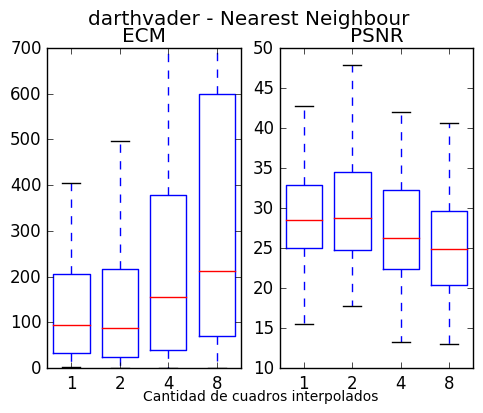
\includegraphics[width=1\textwidth]{imgs/resultados_error/darthvader_0.png}
\end{minipage}%
\begin{minipage}{0.35\textwidth}   
    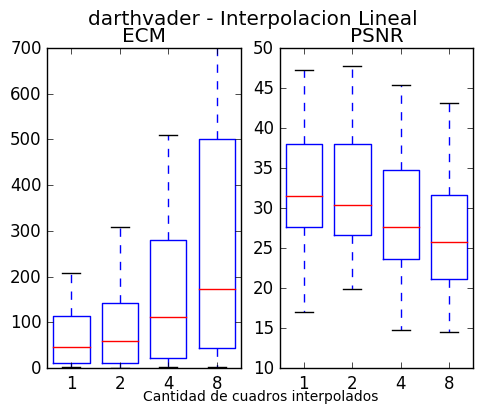
\includegraphics[width=1\textwidth]{imgs/resultados_error/darthvader_1.png} 
\end{minipage}
\end{figure}
\begin{figure}[H]
\centering
\begin{minipage}{0.33\textwidth}   
    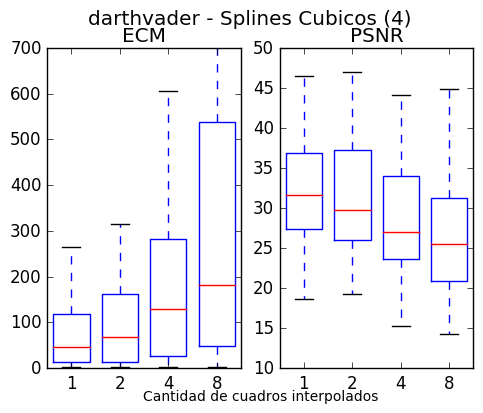
\includegraphics[width=1\textwidth]{imgs/resultados_error/darthvader_2.png} 
\end{minipage}\hfill
\begin{minipage}{0.33\textwidth}   
    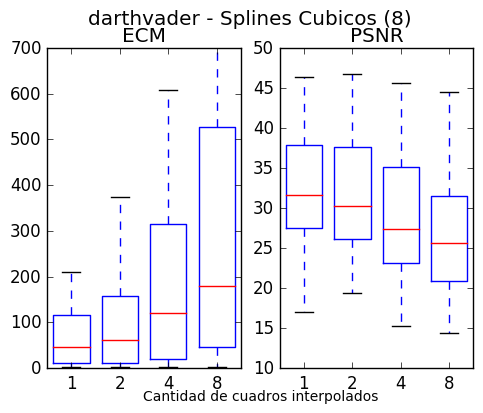
\includegraphics[width=1\textwidth]{imgs/resultados_error/darthvader_3.png} 
\end{minipage}\hfill
\begin{minipage}{0.33\textwidth}   
    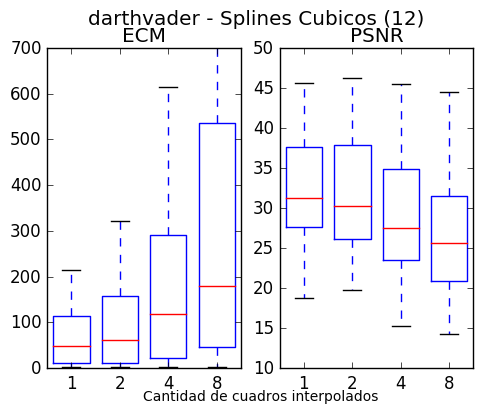
\includegraphics[width=1\textwidth]{imgs/resultados_error/darthvader_4.png} 
\end{minipage}
\caption{\footnotesize Resultados del cálculo de ECM y PSNR para cada algoritmo en el video \texttt{darthvader}. Para Splines cúbicos se indica además el tamaño de los bloques utilizados.}
\end{figure}


\begin{figure}[H]
\centering
\begin{minipage}{0.35\textwidth}
    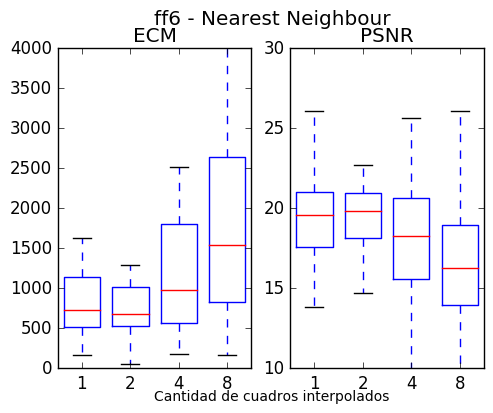
\includegraphics[width=1\textwidth]{imgs/resultados_error/ff6_0.png}
\end{minipage}%
\begin{minipage}{0.35\textwidth}   
    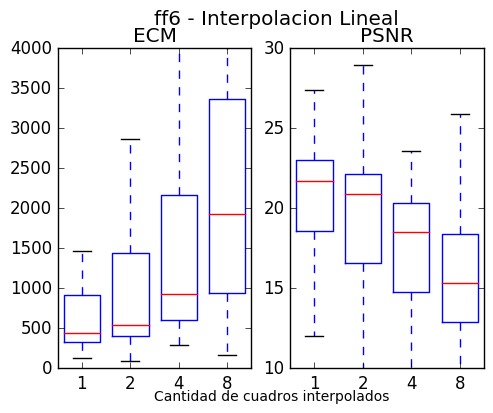
\includegraphics[width=1\textwidth]{imgs/resultados_error/ff6_1.png} 
\end{minipage}
\end{figure}
\begin{figure}[H]
\centering
\begin{minipage}{0.33\textwidth}   
    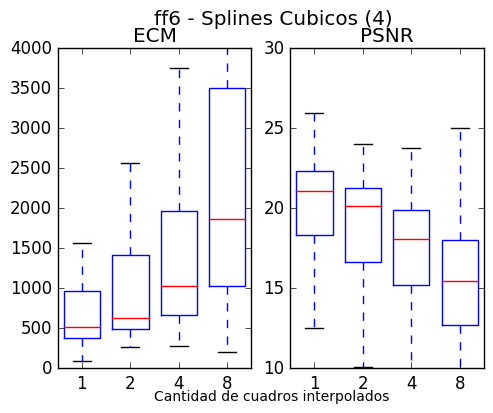
\includegraphics[width=1\textwidth]{imgs/resultados_error/ff6_2.png} 
\end{minipage}\hfill
\begin{minipage}{0.33\textwidth}   
    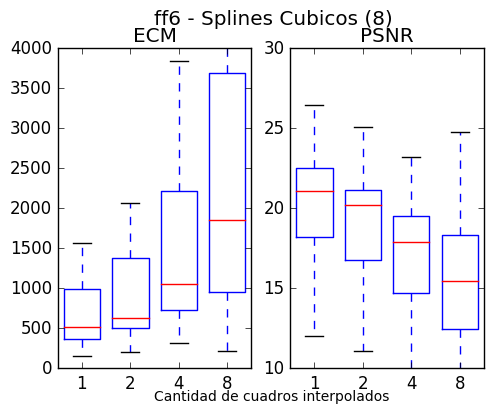
\includegraphics[width=1\textwidth]{imgs/resultados_error/ff6_3.png} 
\end{minipage}\hfill
\begin{minipage}{0.33\textwidth}   
    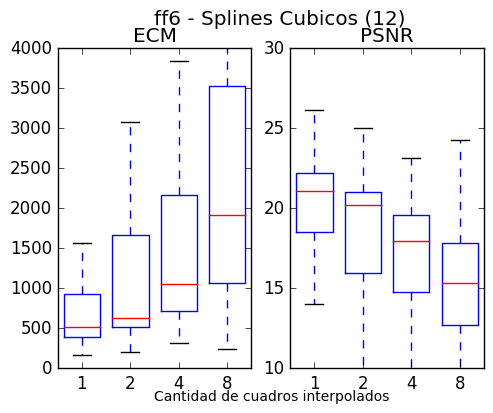
\includegraphics[width=1\textwidth]{imgs/resultados_error/ff6_4.png} 
\end{minipage}
\caption{\footnotesize Resultados del cálculo de ECM y PSNR para cada algoritmo en el video \texttt{ff6}. Para Splines cúbicos se indica además el tamaño de los bloques utilizados.}
\end{figure}


\begin{figure}[H]
\centering
\begin{minipage}{0.35\textwidth}
    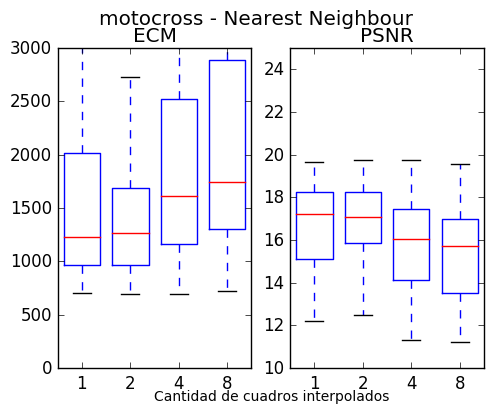
\includegraphics[width=1\textwidth]{imgs/resultados_error/motocross_0.png}
\end{minipage}%
\begin{minipage}{0.35\textwidth}   
    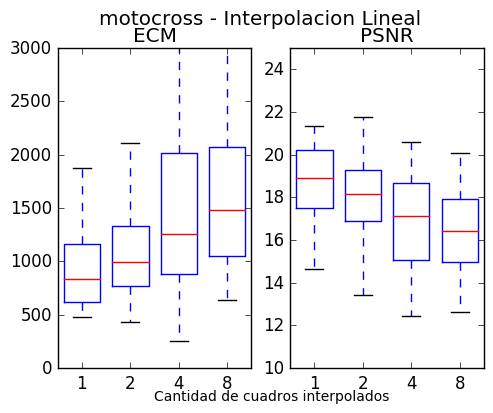
\includegraphics[width=1\textwidth]{imgs/resultados_error/motocross_1.png} 
\end{minipage}
\end{figure}
\begin{figure}[H]
\centering
\begin{minipage}{0.33\textwidth}   
    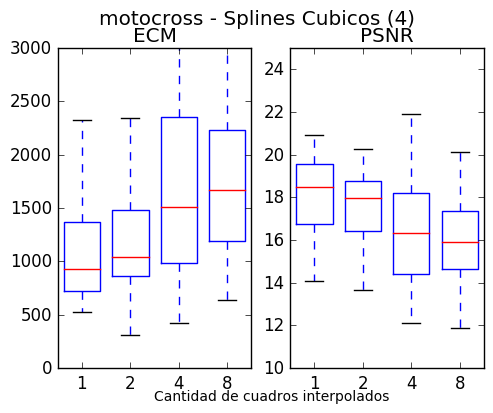
\includegraphics[width=1\textwidth]{imgs/resultados_error/motocross_2.png} 
\end{minipage}\hfill
\begin{minipage}{0.33\textwidth}   
    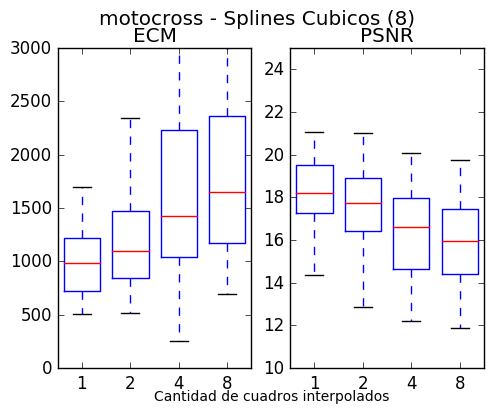
\includegraphics[width=1\textwidth]{imgs/resultados_error/motocross_3.png} 
\end{minipage}\hfill
\begin{minipage}{0.33\textwidth}   
    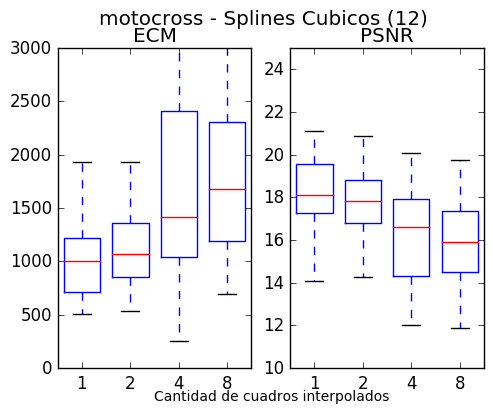
\includegraphics[width=1\textwidth]{imgs/resultados_error/motocross_4.png} 
\end{minipage}
\caption{\footnotesize Resultados del cálculo de ECM y PSNR para cada algoritmo en el video \texttt{motocross}. Para Splines cúbicos se indica además el tamaño de los bloques utilizados.}
\end{figure}


\begin{figure}[H]
\centering
\begin{minipage}{0.35\textwidth}
    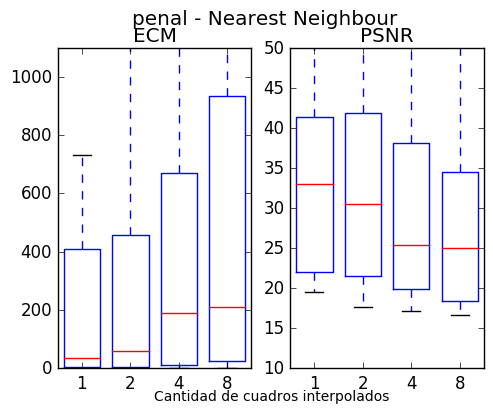
\includegraphics[width=1\textwidth]{imgs/resultados_error/penal_0.png}
\end{minipage}%
\begin{minipage}{0.35\textwidth}   
    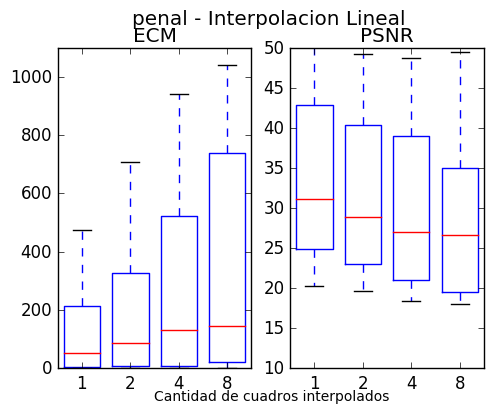
\includegraphics[width=1\textwidth]{imgs/resultados_error/penal_1.png} 
\end{minipage}
\end{figure}
\begin{figure}[H]
\centering
\begin{minipage}{0.33\textwidth}   
    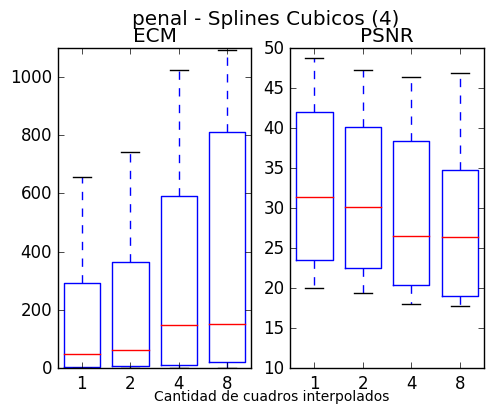
\includegraphics[width=1\textwidth]{imgs/resultados_error/penal_2.png} 
\end{minipage}\hfill
\begin{minipage}{0.33\textwidth}   
    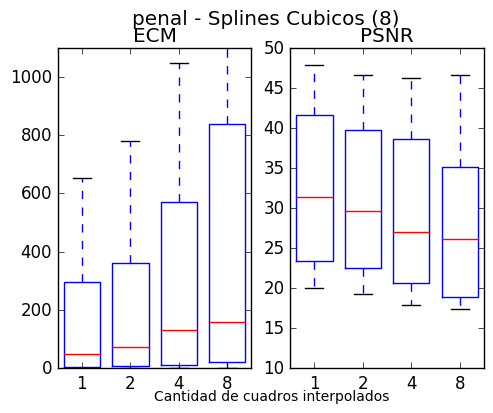
\includegraphics[width=1\textwidth]{imgs/resultados_error/penal_3.png} 
\end{minipage}\hfill
\begin{minipage}{0.33\textwidth}   
    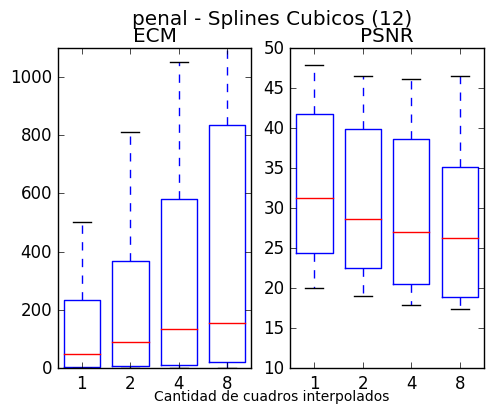
\includegraphics[width=1\textwidth]{imgs/resultados_error/penal_4.png} 
\end{minipage}
\caption{\footnotesize Resultados del cálculo de ECM y PSNR para cada algoritmo en el video \texttt{penal}. Para Splines cúbicos se indica además el tamaño de los bloques utilizados.}
\end{figure}

